\chapter{Entwurf und Implementierung}
\label{cha:implementierung}

In diesem Kapitel legen wir die Grundlagen für einen praktischen Test unserer Forschungshypothese und entwickeln aus den bisherigen Anforderungen eine Brokering-Strategie und einen Architekturvorschlag. Wir definieren außerdem kombinierte, formale Schemata für Anwendungsvorlagen und Qualitätsvereinbarungen. Anschließend geben wir eine Einführung in Multi-Cloud-Bibliotheken und die Python-Ent\-wick\-lungs\-um\-ge\-bung unseres Prototyps.

\section{Brokering-Strategie}
\label{sec:brokering}

Der Broker soll die einzelnen Services einer Anwendung auf die verfügbaren Cloud-Ressourcen verteilen. Dabei muss er die verschiedenen Anforderungen der Anwendung und der benutzerdefinierten Qualitätsziele beachten, um eine erste Vorauswahl geeigneter Clouds zu treffen. Anschließend muss diese Liste anhand weiterer Kriterien optimiert und priorisiert werden. Hierzu zeigen wir mehrere Ansätze und entwickeln eine Strategie für den Multi-Cloud-Broker, die wir anhand von Pseudocode erläutern.

Zu Beginn der Servicemodellierung müssen minimale Hard- und Softwareanforderungen definiert werden. Der Scheduler bildet diese Anforderungen später auf geeignete Cloud-Instanzen der verschiedenen Anbieter ab. Weitere harte Kriterien sind Geo-Standorte anhand der Gesetzgebung, Verschlüsselung und Redundanz. Hinzu kommen dynamische SLO-Metriken wie die Latenz aus verschiedenen Regionen, Durchsatz als Anfragen pro Sekunde und die tatsächliche Verfügbarkeit. Um die Ressourcennutzung zu optimieren, bevorzugen wir eigene Infrastruktur der Private-Clouds. Aus den geeigneten Drittanbietern wählen wir den jeweils günstigsten.

\begin{listing}[ht]
\begin{minted}{python}
def place_service(clouds, service_template, sla):
  req_instance_types = service_template.instances
  req_regions = sla.regions
	
  offered_clouds = filter(c.instance in req_instance_types, clouds)
  offered_regions = filter(c.location in req_regions, offered_clouds)
	
  offered_prices = sorted(offered_regions, key=k['price'])
  allocated_place = offered_prices[0]
	
  if allocated_place is None:
    raise SchedulerError("No match. Check resources or change SLA.")
  else:
    return allocated_place
\end{minted}
\caption{Algorithmus zur Service-Platzierung: Aus der Liste verfügbarer Clouds werden die technisch und regulatorisch geeigneten ausgewählt. Anschließend wird der Service innerhalb des günstigsten Angebots platziert.}
\label{listing:placing}
\end{listing}

\begin{listing}[ht]
\begin{minted}{python}
def scale(clouds, app_template, sla):
  running_instances = filter_by_app(app_template, clouds)
  idle_instances = filter(has_no_connection(i), running_instances)
	
  is_replicated = len(running_instances) >= sla.replication_factor
  is_overprovisioned = len(running_instances) >= sla.replication_factor + 1
  meets_throughput = benchmark(app_template, sla) >= sla.throughput

  if meets_throughput and is_overprovisioned:
    expensive_idle = sorted(idle_instances, key=i['price'], reverse=True)
    expensive_idle[0].shutdown()
  elif not is_replicated or not meets_throughput:
    place_service(clouds, service_template, sla)
\end{minted}
\caption{Vereinfachter Algorithmus zur horizontalen Skalierung einer verteilten Anwendung. Sollte der Cluster die Mindestredundanz sowie alle Leistungsvereinbarungen übertreffen, kann eine Instanz zur Kosteneinsparung heruntergefahren werden. Sinnvollerweise sollte dies die Teuerste sein. Bei Nichterfüllung der Anforderungen beauftragen wir den Scheduler einen geeigneten Platz für eine weitere Instanz zu finden. Nicht abgebildet: die Auflösung von internen Service-Abhängigkeiten.}
\label{listing:scaling}
\end{listing}

Dabei nehmen wir folgende Vereinfachungen an: Der Broker wählt die passenden Ressourcen zum Start der Services und skaliert sie anschließend horizontal mithilfe statischer VM- und Containergrößen. Die Lastverteilung von Clientanfragen übernimmt die Anwendung selbst. Statt simpler Schwellwerte für CPU- oder RAM-Auslastung nutzen wir die SLO-Metrik beantwortete Anfragen pro Sekunde, die in jedem Brokerdurchgang geprüft wird.

Zur Auswahl des Hosts aus der Liste aller vorgefilterten Clouds existieren aufwendige Methoden, wie möglichst niedriger Latenz oder hoher Zuverlässigkeit. Wir nutzen stattdessen diese Möglichkeiten; der Host mit niedrigster CPU-/RAM-Auslastung oder Container-Anzahl \emph{(Spread)}, der Host mit höchster Auslastung \emph{(Binpack)}, eine zufällige Auswahl \emph{(Random)}, oder die Cloud mit den niedrigsten erwarteten Kosten \emph{(Cheapest)}.

Selbst die Kostenberechnung eines einzelnen Anbieters ist komplex: Je nach Abnahmemenge und Vertragslaufzeit können die Preise stark variieren\footnote{\url{https://www.rightscale.com/blog/cloud-cost-analysis/aws-vs-azure-vs-google-cloud-pricing-compute-instances}}. Zusatzkosten können durch den Datentransfer außerhalb eines Anbieters entstehen. Diese Preisstrukturen stehen den Zielen Portabilität und Ausfallsicherheit entgegen, denn die geringsten Kosten fallen bei dem Betrieb in einer einzelnen Cloud eines Providers an. Für den Prototyp beschränken wir uns trotzdem auf die Berechnung der Rechenkapazität und des Speicherplatzes. Den Platzierungsprozess zeigt Listing \ref{listing:placing}.

Die Leistung eines Rechenknotens der Cloud-Provider kann sich durch Updates und Rekonfigurationen signifikant ändern -- aber auch, sobald die Aufgaben der Nachbar-VMs wechseln. Daher gibt es Machine-Learning-Ansätze, um die Performance-Charakteristika einer Anwendung und eines bestimmten Infrastrukturknotens zu \emph{lernen}. Hierdurch kann die optimale Angebotsgröße der Provider gewählt werden, um weitere Kosteneinsparungen zu erreichen \cite{grozev:2016:ml-brokering}. Ein klassischerer Ansatz sind Simulationen und Graph-basierte Ansätze. Gleiches ist für die Verfügbarkeit eines bestimmten Anbieters denkbar: Wie zuverlässig war das Angebot wirklich? Ist eine Entschädigung fällig? Möglicherweise kann die Anzahl der Provider reduziert werden, solange die minimale Replikationsstufe nicht unterschritten wird. Den Algorithmus hierzu zeigt Listing \ref{listing:scaling}.

Ob einzelne Instanzen sich einfach stoppen lassen, ist allerdings abhängig vom Anwendungsmodell: Zustandslose Architekturen sind einfacher zu handhaben. Für sitzungsgetriebene Anwendungen ist eine Zusammenarbeit mit Lastverteilungssystemen denkbar. Diese könnten, unter Beachtung der Qualitätskriterien, alle Verbindungen auf möglichst wenige Hosts bündeln. Auch messbar ist die Bootzeit eines bestimmten Providers. Wie elastisch ist das Angebot? Mit welcher Kombination aus Anbietern kann eine akzeptable Wiederherstellungszeit erreicht werden? Dies sind mögliche Aspekte weiterer Forschung. Aktuell ist die Strategie für Brokering und automatischer Skalierung reaktiv, aber noch nicht vorausschauend oder proaktiv. Wir erwarten trotzdem eine Erhöhung von Ausfallsicherheit und Portabilität. Der folgende Abschnitt zeigt die Broker-Architektur.


\section{Modularer Architekturvorschlag}
\label{sec:architektur}

%Komponenten des Brokers.
%
%
%In der CMP: Polling oder Notification?
%
%Was löst eine Aktion aus?
%- Monitoring der Services
%- Änderung der Umgebung
%- User-Aktion
%- Ergebnis einer anderen Policy

\begin{figure}
	\centering	
%	\def\svgwidth{0.95\textwidth}
%	{\tiny
%	\includesvg{images/broker-cycle}}
	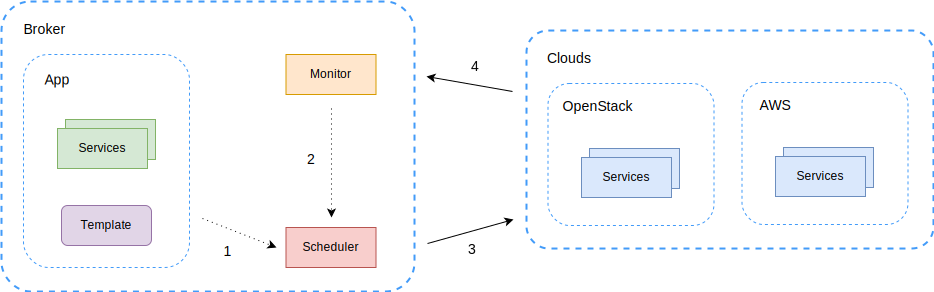
\includegraphics[width=\linewidth]{images/broker-cycle}
	\caption{Arbeitsweise des Multi-Cloud-Brokers als Zyklus: (1) Sammeln der Meta-Informationen aller Cloud-Provider, (2) Sammeln der Laufzeitinformationen der Anwendungen, (3) Sammeln der SLAs, (4) Nutzeränderungen: Neue Anwendungen oder Anpassung von SLAs, (5) Optimierungsplanung, (6) Planausführung auf den Cloud-Infrastrukturen}
	\label{fig:cycle}
\end{figure}

%Zyklus\autoref{fig:cycle}:

%\begin{description}
%	\item[Nummerierte Aufzählung]~\par
\begin{enumerate}
	
	\item Sammeln der Meta-Informationen alle Cloud-Provider
	\begin{enumerate}
		\item Kapazität (CPU, RAM, HDD, Network)
		\item Features (Verschlüsselung, CUDA, …)
		\item Geo-Lokation 
		\item Preis
	\end{enumerate}
	
	\item Sammeln der Laufzeitinformationen der PaaS/Anwendungen
	\begin{enumerate}
		\item Auslastung
		\item Fehler
		\item Ausfälle
	\end{enumerate}
	
	\item Sammeln der SLAs
	\begin{enumerate}
		\item Policy-Definitionen
		\item Policy-Konfiguration
		\item Placement-Algorithmen
	\end{enumerate}
	
	\item Neue Anwendung/Änderung eines SLA
	
	\item Optimierung
	\begin{enumerate}
		\item Feste Vorgaben (Geo, Backup)
		\item Weiche (Preis, Latenz, Verfügbarkeit)
	\end{enumerate}
	
	
	\item Ausführung
	\begin{enumerate}
		\item Netzwerkkonfiguration
		\item Allokation/De-Allokation von Ressourcen
		\item Deployment
		\item Migration
		\item Logging/Benachrichtigung
		\item Backup
	\end{enumerate}
	
\end{enumerate}

\section{Multi-Provider-Service-Schema}

Konfigurationsdateien sind im aktuellen Prototyp die einzige Benutzerschnittstelle. Sie liefern vielfältige Angaben: 

\begin{enumerate}
	\item Cloud-Provider-Zugangsdaten und -Metainformationen
	\item Service-Topologie, -Definition und -Konfiguration
	\item Service-Level-Objective-Anpassungen
\end{enumerate}

Alle nutzeranpassbaren Dateien folgen der vereinfachten Auszeichnungssprache YAML \emph{(YAML Ain't Markup Language)} zur datenorientierten Speicherung mithilfe von (assoziativen) Listen und Einzelwerten. Im Gegensatz zu XML oder JSON sind die resultierenden Konfigurationsdateien für Menschen einfacher lesbar. Gleichzeitig existieren Interpreter für alle verbreiteten Sprachen und Systeme. Durch die zeilenbasierte Speicherung einzelner Werte sind YAML-Dateien außerdem über Git versionierbar. Entsprechend hat sich der YAML-Standard als Konfigurationssyntax im Cloud- und DevOps-Kontext durchgesetzt; genutzt wird er zum Beispiel auch von AWS-Angeboten, Docker Compose oder Travis-CI. Als offener, menschen- und maschinenlesbarer Standard erfüllt YAML das Versprechen von Portabilität.

\begin{listing}[ht]	
	\inputminted[]{yaml}{./src/provider.sample.yaml}
	\caption{Provider-Definition und Zugangsdaten. Der Broker liest alle eingetragenen Accounts automatisch ein und berücksichtigt sie bei der initialen Service-Bereitstellung sowie in Optimierungsläufen. Public-Clouds benötigen nur Zugangsdaten wie Benutzername und Passwort -- alle weiteren Informationen erfragt der Broker dynamisch zur Laufzeit vom Provider. In Private-Cloud-Umgebungen ist dies nicht immer möglich: Details zur Verfügbarkeit, geografische Lage und Kosten müssen manuell eingepflegt oder vom Monitoring festgestellt werden.}
	\label{listing:provider}
\end{listing}

Ausschnitt \ref{listing:provider} zeigt die Definition der Serviceprovider: Public-Cloud-Angebote benötigen nur Angaben zur Authentifizierung, alle weiteren Informationen ruft Libcloud dynamisch zur Laufzeit ab. Dies können zum Beispiel aktuelle Preisinformationen, verfügbare Ressourcen und Geostandorte sein. Für private Infrastrukturen müssen diese Daten möglicherweise manuell eingetragen werden -- es liegt an den IT-Verantwortlichen, die anfallenden Kosten einer OpenStack-Instanz zu berechnen. Verfügbarkeitsstatistiken können direkt hinterlegt oder vom Broker berechnet werden. Obligatorisch ist die Angabe eines technischen Providers wie \emph{docker} oder \emph{ecs} und einer eindeutigen ID.

Services und SLOs sollen providerübergreifend, abstrakt definiert werden. In \autoref{sec:service-definition} haben wir hierzu den Standard TOSCA ausgewählt: Durch zweckmäßige Basistypen und Vererbung lassen sich übliche Webanwendungstopologien mit Qualitätsvereinbarungen kombinieren. Auch hier können wir YAML einsetzen -- dazu implementieren wir eine Untermenge von TOSCA-Simple. Wir definieren Basistypen für Services und importierbare Qualitätsziele. Nutzer können anschließend eigene Wünsche einbringen: Sie ergänzen durch Importe oder überschreiben Werte und Variablen manuell. Ausschnitt \autoref{listing:hyrise-r} zeigt die Definition für einen Hyrise-R-Dispatcher. Alle verbliebenen Variablen füllt der Broker dynamisch während der Planumsetzung. Zum Beispiel legt er fest, welcher Service-Teil, auf welchem Provider, mit welchem Instanz-Typen, bereitgestellt wird. Technisch basieren die Variablen auf der Jinja2-Syntax. 

Ausgeführte Pläne speichert der Broker mit ausgefüllten Variablen, Anwendungskennung und einer UUID als YAML-Dokumentation. Denkbar wäre auch eine Sicherung des Brokerergebnisses als CAMP-Plan, dieser wäre kompatibel mit anderen offenen Cloud-Management-Systemen. Diese Kooperation könnte ein Thema für weitere Arbeiten sein. Der Broker vergibt den gestarteten Instanzen außerdem Metainformationen als Labels, der Betrieb ist also theoretisch zustandslos: Aus den Zugangsinformationen zur Cloud-Infrastruktur und den Informationen der gestarteten Instanzen lassen sich die Anwendungen jederzeit rekonstruieren. Die Basisdefinitionen der Services liefern weitere Instruktionen zur Zustandsprüfung auf Service-Ebene und Reaktionen im Fehlerfall. Die folgende Auflistung erläutert alle Bestandteile unserer providerübergreifenden Servicedefininition:


\begin{description}
	
	\item[Kommentare] sind innerhalb der Service-Definition nicht vorgesehen. Mit einer Ausnahme: Eine Einleitung zu Art und Verwendung der YAML-Datei ist erlaubt. In diesem Fall handelt es sich zum Beispiel um eine Jinja2-Vorlage, die unterhalb des Verzeichnisses \emph{services/} platziert werden sollte.
	
	\item[Metadaten] Jede Service-Definition enthält eine Präambel aus verschiedenen Metadaten. Der Broker benötigt als erste Information eine Schema-Version. Zum Zeitpunkt der Arbeit existiert nur die Definition 1.0, dies könnte sich in Zukunft natürlich ändern, und sollte semantisch versioniert werden. Darüber hinaus ist auch der Inhalt eines Service-Schemas versioniert und datiert. 
	
	Die Informationen zu Autor und Lizenz sind für den Broker nicht wichtig, sie ermöglichen aber die Veröffentlichung eines Schemas in einem Cloud-übergreifenden Service-Katalog. Unterstützend sind die Links zu Quellcode, Website und Logo der integrierten Anwendung zusammen mit einer Kurzbeschreibung.

	\item[Importe] Aus TOSCA stammt die Idee von Service-Komponenten und -Klassen sowie Policy-Templates, die über einfache YAML-Importe eingebunden werden. Vorteil ist die schnellere Entwicklungszeit eines konkreten Services, nach dem \emph{DRY}-Prinzip. Die Importfunktion ist außerdem unabhängig vom Broker: Sie entspricht dem YAML-Standard. Der Verwaltungsaufwand verlagert sich allerdings, sobald die Vorlagen Service-übergreifend definiert werden und von der TOSCA-Standarddefinition abweichen.
	
	\item[Topologie] YAML-Auschnitt \autoref{listing:hyrise-r} zeigt den Inhalt der Liste \emph{services}: Sie enthält alle Anwendungskomponenten, die jeweils einzeln gestartet werden müssen. Jede Komponente hat eine eindeutige ID, hierüber lassen sich Attribute referenzieren.
	
	Ein Hyrise-Cluster besteht immer aus genau einem Dispatcher und genau einem Master -- beide Services sind entsprechend als \emph{global} gekennzeichnet. Dagegen sind Replica-Knoten optional und können in beliebiger Anzahl ergänzt werden. \emph{depends\_on} definiert diese Abhängigkeiten untereinander: Der Master benötigt einen gestarteten Dispatcher zur Registrierung. Replicas erwarten zusätzlich einen Master, um den Datenbestand abzugleichen.	
	
	\item[Laufzeitumgebung] und Konfigurationsschnittstelle unterschieden sich je nach Provider. Für Docker definieren wir ein Container-Image zum Download aus dem zentralen Docker Hub. Sowohl lokale Installationen als auch Cloud-Container-Dienste beziehen ihre Images hieraus. OpenStack besitzt den eigenen Image-Dienst \emph{Glance} -- ist ein Image noch nicht vorhanden, laden wir es bei Bedarf hoch.
	
	Die Erstkonfiguration erfolgt über den Docker Entrypoint beziehungsweise cloud-init. In beiden Fällen sind die Konfigurationsvariablen zu IP-Adressen, Ports und IDs in \emph{Jinja2}-Syntax angelegt. Der Broker füllt sie dynamisch während der Planung.
	
	\item[Ressourcen] Jeder Service benötigt ein Minimum an zugeteilten Ressourcen; CPU-Leistung, Netzwerkbandbreite, RAM- und HDD-Größe. Für Spezialanwendungen kommen noch besondere Anforderungen wie GPU-Funktionen oder FPGA-Zugriff hinzu. Besonders im Fall von Docker können außerdem erweiterte Rechte notwendig sein, die ein Standardcontainer nicht erhält. 
	
	Ist der erhöhte Ressourcenbedarf einer Anwendung von vornherein bekannt, kann das Template entsprechend angepasst werden. Auch die Angabe eines Ressourcenmaximums ist sinnvoll: Kaum ein Service skaliert effizient mit unbegrenzt vielen CPU-Kernen.
	
	\item[Netzwerk] Zur Kommunikation mit anderen Services, Endbenutzern und der Cloud-Management-Plattform benötigen Anwendungen Netzwerkzugriff. Sinnvoll ist eine Trennung der verschiedenen Belange in unabhängigen Netzwerken. Durch die VPN-Integration vieler Infrastrukturanbieter lässt sich diese Anforderung umsetzen. 
	
	Vordefiniert sind die Netzwerke \emph{Frontend} und \emph{Backend}. Ersteres ist in der Standardeinstellung für Nutzer von außerhalb erreichbar, Letzteres dient der Administration und dem Datenaustausch zwischen den Services selbst.
		
	\item[Wartung] Im Gegensatz zu einem einfachen Broker kümmert sich die Cloud-Management-Plattform auch um den ordnungsgemäßen Weiterbetrieb einer Anwendung. Wir definieren daher eine rudimentäre Überprüfung der Funktionsfähigkeit: In einem bestimmten Intervall soll die CMP eine HTTP-Schnittstelle ansprechen. Kommt auch nach drei Versuchen keine gültige Antwort, gilt die Service-Instanz als verloren und wird neu gestartet. Über weitere SLOs lässt sich das Verhalten anpassen. Für Hyrise existiert kein Stopp-Kommando: Der Dispatcher erkennt abgeschaltete Knoten selbstständig.
	
\end{description}

\begin{listing}[ht]	
	\inputminted[firstline=15]{yaml}{./src/hyrise-r.sample.yaml}
	\caption{Providerübergreifende Servicevorlage. Der Ausschnitt zeigt die Definition des zentralen \emph{Hyrise-R-Dispatcher}-Dienstes. Nicht zu sehen sind Metadaten und die übrigen Anwendungsbestandteile. Parameter werden zur Laufzeit vom Broker eingesetzt.}
	\label{listing:hyrise-r}
\end{listing}

Am Beispiel von OpenStack, AWS und Hyrise-R haben wir die Definition von providerübergreifenden Services und Qualitätsvereinbarungen in einem offenen YAML-Standard beschrieben. Das nächste Kapitel zeigt eine konkrete Teststellung und versucht unsere Forschungshypothese zu validieren.

\section{Multi-Cloud-Bibliotheken}
\label{sec:bibliotheken}

Ziel ist die Implementierung eines externen Broker-Services für den automatischen Betrieb mit mehreren Clouds. Da unabhängige Cloud-Provider keine einheitlichen APIs anbieten, stellt dieses Kapitel verschiedene Bibliotheken vor, um möglichst viel der zusätzlichen Komplexität zu verbergen, siehe \autoref{fig:multi-cloud-library}.

Ohne weitere Bibliotheken müsste für jede zu berücksichtigende Cloud das jeweilige SDK eingebunden werden. Auch Namensgebung, Architektur und Prozesse unterscheiden sich von Anbieter zu Anbieter.

\begin{figure}[ht]
%\begin{wrapfigure}{O}{0.3\textwidth}
	\centering
%	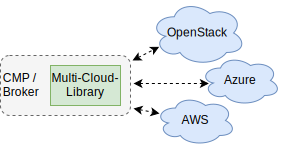
\includegraphics[width=0.48\textwidth]{images/multi-cloud-library.pdf}
		\def\svgwidth{0.48\textwidth}
		{\scriptsize \textsf{
		\includesvg{images/multi-cloud-library}}}
	\caption{Eingebette Bibliothek zur Multi-Cloud-Kommunikation.}	
	\label{fig:multi-cloud-library}
%\end{wrapfigure}
\end{figure}

Durch den Einsatz einer Drittbibliothek ergibt sich allerdings eine potenzielle Schwachstelle. Falls die Bibliothek fehlerhaft ist -- oder nicht weiter entwickelt wird -- gefährdet sie das gesamte Projekt. Historie und Zukunftschancen spielen bei der Auswahl eine zentrale Rolle. Im Optimalfall abstrahiert die Bibliothek alle zukünftigen Änderungen der Provider-SDKs. Ob und wie groß die Arbeitserleichterung ausfällt, prüft der Praxisteil.

Im Folgenden untersuchen wir die Eignung der populärsten Bibliotheken. Wichtigste Komponente ist dabei das Computing-Modul. Wünschenswert wäre auch Container-Unterstützung, um Images anbieterunabhängig bereitzustellen. Gestartete Anwendungskomponenten erfordern für die erste Erreichbarkeit oft Zugriff auf die DNS-Einstellungen der Cloud. Optional ist die Unterstützung von \emph{Content Delivery Networks}, Speicher- und Sicherungs-Diensten.


% https://tex.stackexchange.com/questions/341592/hyphenating-text-inside-tabularx
\begin{table*}\centering
	\begin{minipage}{\textwidth}
		\caption{Übersicht freier Multi-Cloud-Bibliotheken. Mit $*$ gekennzeichnete Eigenschaften sind experimentell. Aufgeführt sind nur die populärsten Cloud-Provider, die Bibliotheken können darüber hinaus weitere unterstützen. Ob eine Bibliothek weitere Informationen, wie aktuelle Preisinformationen und den Standort des Rechenzentrums abrufen kann, zeigt die Spalte \emph{Cost\,/\,Geo}.}
		\ra{1.3}
		\begin{tabularx}{\textwidth}{LLLr} \toprule
			Projekt & Cloud-Provider & Cloud-Services & Cost\,/\,Geo\\ \midrule
			Apache Libcloud (Python)\footnotemark & AWS, Azure, OpenStack, GCP, Docker & Compute, Container, DNS, Load Balancer, Storage, Backup & $x$\,/\,$x$\\
			Apache jclouds (Java)\footnotemark & AWS, Azure, Open\-Stack$*$, GCP, Docker & Compute, Container, Load Balancer$*$, Storage & $x$\,/\,$x$\\
			PkgCloud (Node.js)\footnotemark & AWS, Azure, OpenStack& Compute, Load Balancer, Storage$*$, DNS$*$ & --\,/\,--\\
			Libretto (Go)\footnotemark & AWS, Azure, OpenStack, GCP & Compute & --\,/\,--\\
			Fog (Ruby)\footnotemark & AWS, OpenStack, GCP & Compute, DNS, Storage & $x*$\,/\,--\\
			\bottomrule
		\end{tabularx}
		\label{tab:bibliotheken}
		\vspace{150pt}
		\footnotetext[1]{\url{https://libcloud.apache.org/}}
		\footnotetext[2]{\url{https://jclouds.apache.org/}}
		\footnotetext[3]{\url{https://github.com/pkgcloud/pkgcloud/}}
		\footnotetext[4]{\url{https://github.com/apcera/libretto/}}
		\footnotetext[5]{\url{http://fog.io/}}
	\end{minipage}
\end{table*}

\autoref*{tab:bibliotheken} listet die untersuchten Bibliotheken mit unterstützten Cloud-Providern, Diensten und weiteren Funktionen. Letzteres sind Zugriff auf Preisinformationen des Anbieters und Standortinformationen der Rechenzentren. Zusätzlich sollten die Projekte kontinuierlich weiterentwickelt werden, eine aktive Entwicklergemeinschaft besitzen und gut dokumentiert sein. Alle sind quelloffen und unter einer freien Lizenz verfügbar.

\begin{description}
	
	\item[Apache jclouds] existiert schon seit 2009. Es unterstützt zumindest experimentell die wichtigsten Provider, aber nicht alle Dienste. So ist DNS nicht vorhanden, Container-Unterstützung gibt es nur für Docker. Die Bibliothek ist gut getestet, dokumentiert, und mit zahlreichen Beispielen ausgestattet. Durch Java ist sie außerdem typsicher. 
	
	\emph{jclouds} ist zudem Grundlage mehrerer Multi-Cloud-Projekte, z.\,B. von \emph{Apache brooklyn\footnote{\url{https://brooklyn.apache.org/}}}, das mithilfe von \emph{CAMP}-Plänen Anwendungen über mehrere Clouds ausrollt.
	
	\item[Apache Libcloud] vereint eine Reihe von Vorteilen: Es unterstützt neben OpenStack -- als Referenz für Private-Cloud-Installationen -- sämtliche großen und kleinen Cloud-Provider mit allen Kernfunktionen. Besonders interessant ist die Container-Unterstützung für \emph{Docker}, \emph{Kubernetes}, \emph{Amazon ECS} und die \emph{Google Container Engine}. Entsprechend gepackte Anwendungen könnten in einer Vielzahl von Clouds ohne weitere Änderungen ausgeführt werden.
	
	\item[Fog] integriert die wichtigsten Anbieter und Dienste. Die Entwicklergemeinde rund um \emph{Fog} ist aktiv und die Bibliothek wird häufig eingesetzt. Besonders interessant sind die bereitgestellten Mocks, die als Platzhalter Tests neuer Integrationen erleichtern sollen. Zumindest für OpenStack wird Metering unterstützt, also die Abfrage bisher in Anspruch genommener Ressourcen. Eine einheitliche Namensgebung der verschiedenen Cloud-Produkte existiert nicht.
	
	\item[Libretto] beschränkt sich ausdrücklich auf die Compute-Funktionalität mithilfe virtueller Maschinen. Das zugehörige Projekt ist aktiv, kommt aufgrund der fehlenden Funktionalität aber nicht infrage.
	
	\item[PkgCloud] ist die einzige bekannte \emph{Node.js}-Bibliothek. Funktionsumfang und einheitliche Namensgebung der Cloud-Services sind überzeugend; leider wird die Bibliothek seit dem Verkauf des federführenden Unternehmens nicht mehr aktiv gepflegt. Bereits eingereichte Pull Requests werden nicht bearbeitet. Damit scheidet \emph{PkgCloud} für das Projekt aus.
	
\end{description}

\noindent Vielversprechend war außerdem das \emph{Apache-DeltaCloud}-Projekt: Aufbauend auf \emph{Ruby} stellt es nicht nur eine einheitliche API nach \emph{Cloud-Infrastructure-Management-Interface}-Standard\footnote{\url{https://www.dmtf.org/standards/cloud}} für die Kernfunktionen der wichtigsten Cloud-Provider, sondern auch zusätzliche Client-Bibliotheken und Mock-Funktionen. Aufgrund des plötzlichen Rückzugs von \emph{Red Hat} erfolgt seit 2013 allerdings keine Weiterentwicklung mehr \cite{androu:2013:deltacloud-red-hat-end}. Dieses Beispiel zeigt die Relevanz nicht-funktionaler Betrachtungen bei der Auswahl einer Bibliothek. Auch Apache-Top-Level-Projekte haben nicht unbedingt eine sichere, vorhersagbare Zukunft.

Darüber hinaus existieren spezialisierte Bibliotheken wie \emph{SimpleCloud}\footnote{\url{https://framework.zend.com/manual/1.11/de/zend.cloud.html}} auf \emph{PHP}-Basis, das allerdings eine feste Komponente im \emph{Zend Framework} ist. Auch gibt es neue Entwicklungen wie \emph{CloudBridge}\footnote{\url{https://github.com/gvlproject/cloudbridge}} auf \emph{Python}-Basis. Besonderheit hier: Die Abstraktionsschicht nutzt die nativen SDKs der Cloud-Provider. \emph{CloudBridge} ist leider noch in einem frühen Entwicklungsstadium und als experimentell gekennzeichnet.

\emph{Libcloud} fasst die verschiedenen Cloud-Angebote nicht nur in gemeinsamen Namensräumen zusammen, sondern normalisiert auch Leistungsklassen. Python erleichtert außerdem den Einstieg und fügt sich in viele \emph{Python}-basierte Systemautomatisierungen ein. Diese Multi-Cloud-Bibliothek wird also im weiteren Verlauf der Arbeit erprobt.

%https://brooklyn.apache.org/learnmore/theory.html
% Apache Brooklyn hat eine eigene YAML-Service-Description-Spezifikation, ähnlich zu CAMP, der Clou Application Management API. Die Integration von TOSCA ist geplant, und in einer anderen Arbeit bereit umgesetzt: 
%Trans-Cloud: CAMP/TOSCA-based Bidimensional Cross-Cloud
% Keine SLAs, sondern nur Trigger-Action-Policies.
% Nutzt intern jclouds zur Provider-Anbindung.

\section{Softwarearchitektur und Entwicklungsumgebung}

Dieser Abschnitt beschreibt die konkrete technische Umsetzung des Brokers. Die Architektur orientiert sich an den in \autoref{sec:architektur} vorgestellten Komponenten. Die Konfiguration basiert außerdem auf den in \autoref{sec:service-schema} definierten YAML-Schemata für Cloud-Zugänge, Anwendungen und Qualitätsvereinbarungen. Insgesamt soll der Prototyp eine Grundmenge der Brokering-Strategie aus \autoref{sec:brokering} umsetzen --  also eine Anwendung anhand verschiedener Anforderungen auf unterschiedlicher Cloud-Infrastruktur verteilen.

Hierzu haben wir bereits Libcloud als Python-Bibliothek zur Cloud-Abstraktion ausgewählt und nutzen für das gesamte Projekt ausschließlich Python 3.6. Stil-Leitfaden ist PEP\,8\footnote{\url{https://www.python.org/dev/peps/pep-0008/}} zusammen mit einigen bekannten Python-Best-Practices\footnote{\url{http://docs.python-guide.org/en/latest/\#writing-great-python-code}}\footnote{\url{http://pyvideo.org/speaker/raymond-hettinger.html}}. Wir nutzen zum Beispiel \emph{@property} um Getter- und Setter-Methoden zu verbergen; in eigenen Klassen implementieren wir \emph{Magic Methods} wie \emph{\_\_getitem\_\_}. Ganz nach dem \emph{Zen of Python}\footnote{\url{https://www.python.org/dev/peps/pep-0020/}} soll die Implementierung möglichst leicht zu verstehen und zu warten sein.

Alle weiteren Abhängigkeiten installiert der Paketmanager Pipenv\footnote{\url{https://docs.pipenv.org/}} aus dem Pipfile (ähnlich \emph{requirements.txt}), er integriert außerdem \emph{virtualenv} -- der Broker lässt sich so unabhängig von bereits auf Systemebene installierten Python-Versionen und -Modulen  betreiben. Das gesamte Setup und alle Testprozesse sind in einem Makefile zusammengefasst. Außer dem Hyrise-R-Fork und den AWS-/DevStack-Teststellungen enthält das zentrale Broker-Repository folgendes:

\begin{forest}
	pic dir tree,
	where level=0{}{% folder icons by default; override using file for file icons
		directory,
	},
	[%Repository
		[apps/, label=right: Anwendungs- und SLO-Vorlagen{, [*.yaml]}
		]
		[broker/, label=right: Python-Module des Brokers{, [*.py]}
		]
		[doc/, label=right: Diese Thesis{, [*.tex]}
		]
		[test/, label=right: Systemtest{, [*.py]}% siehe \autoref{sec:brokering-test}
		]
		[clouds.yaml, file
		]
		[Makefile, file
		]
		[Pipfile, file
		]
		[Readme.md, file
		]
	]
\end{forest}


\noindent
Der Prototyp ist vereinfacht und demonstriert eine Teilmenge des möglichen Konzeptumfangs. Aus den vorgestellten Aufgaben und dem Brokering-Zyklus ergeben sich im Detail folgende Programmkomponenten, siehe auch  \autoref{fig:broker-architecture}:

\begin{description}
	
	\item[Cloud] ist die Basisklasse für den Zugriff auf Ressourcen. Sie definiert bestimmte Schnittstellen; zum Beispiel die Methode \emph{deploy()}, um aus einer ausgefüllten Vorlage eine Service-Instanz zu starten. Die Klasse verwaltet außerdem Zugangsdaten und den Zugriff auf Qualitätsmetriken, Kosten und Administrationsschnittstellen einer Cloud.
	
	Für jeden Provider existiert eine Adapterklasse, die \emph{Cloud} implementiert und über die jeweiligen Libcloud-Module\footnote{\url{https://libcloud.readthedocs.io/en/latest/supported_providers.html}} die Kommunikation mit Cloud-Providern abwickelt. Unsere Klasse \emph{DockerCloud} nutzt zum Beispiel Libclouds \emph{DockerContainerDriver}. Entsprechendes gilt für OpenStack und AWS. Da alle zentralen Schnittstellen unabhängig vom gewählten Provider bereitstehen, ist der Zugriff für Anwendungen transparent.
	
	\item[App] verwaltet die Verbindungen der einzelnen Anwendungskomponenten mithilfe von Vorlagen: Essenzielle, globale Dienste ohne weitere Abhängigkeiten werden zuerst ausgerollt, dies können zum Beispiel Lastverteilungssysteme sein. Anschließend folgen die Primärdienste, später die redundanten Komponenten. Dabei beachtet \emph{App} die gewünschte Anzahl an Instanzen und beauftragt den Scheduler mit der Suche nach dem passendsten Ressourcen-Anbieter.
	
	\item[Service] Ein Service ist eine einzeln zu startende Komponente einer verteilten Anwendung. Der Zugehörigkeit zu einer größeren Anwendung ist sich die Service-Klasse allerdings nicht bewusst -- Sie ist nur ein Container für die ausgefüllte Vorlage mit Laufzeitkonfiguration und die Verbindung zur ausführenden Cloud.
	
	\item[Template] Cloud-Zugangsdaten und Anwendungsvorlagen liegen als einfache Textdateien mit YAML-Syntax im Verzeichnis des Brokers. Ausgeführte Pläne speichert er zusätzlich im Unterverzeichnis \emph{deployments}. Die genaue Spezifikation hierzu haben wir in \autoref{sec:service-schema} erarbeitet.
	
	Während des Deployments füllt der Broker iterativ alle Platzhalter in den Vorlagen. Beispiel: Nach dem Start eines zentralen Lastverteilungsdienstes ist dessen IP-Adresse bekannt und wird allen weiteren Instanzen mitgegeben. Im Gegensatz zu solchen globalen Variablen speichern wir Parameter redundanter Dienste nur temporär zur Weitergabe an die Infrastruktur-Provider.
	
	Technische Grundlage sind Jinja2\footnote{\url{http://jinja.pocoo.org/}} als Vorlagensprache und ruamel.yaml\footnote{\url{https://yaml.readthedocs.io/en/latest/}} als moderne YAML-Python-Implementierung. Das iterative Ausfüllen der Vorlagen erreichen wir durch die eigene Implementierung der Klasse \emph{IgnoreMissingAttribute}.
	
	\begin{figure}[ht]
		\centering
		\def\svgwidth{0.95\textwidth}
		{\scriptsize \textsf{
				\includesvg{images/broker-architecture}}}
		\caption{Architektur des Python-Prototyps -- Die Klasse \emph{App} verwaltet alle verteilten Komponenten einer Anwendung und deren Qualitätsanforderungen. Diese Forderungen reicht sie an den \emph{Scheduler} weiter, der einen konkreten Deploymentplan entwickelt. Über Provider-spezifische Adapter innerhalb der Klasse \emph{Cloud} werden die Pläne anschließend ausgeführt und überwacht.}
		\label{fig:broker-architecture}
	\end{figure}
			
	\item[Scheduler] nimmt verfügbare Clouds und eine Servicevorlage mit Qualitätskriterien entgegen. Aus der Liste verfügbarer Ressourcen filtert die Planungseinheit alle grundsätzlich passenden Einträge. Anschließend gewichtet er die übrigen Clouds nach weichen Kriterien wie der erwarteten Performance oder dem voraussichtlichen Preis. Das passendste Ergebnis liefert er als konkreten Deploymentvorschlag zurück an die Klasse \emph{App}. Der Scheduler übernimmt gleichzeitig die Funktion des Monitors: Er überprüft in jedem Brokering-Zyklus die vorhandenen Dienste auf Einhaltung der Qualitätskriterien.

	\item[Logger und Tracer] Während des Regelbetriebs würde der Logger komponentenübergreifend alle Ereignisse festhalten. In unserem Prototyp ist die Tracing-Funktion wichtiger: Jede mit \emph{@traced()} dekorierte Methode liefert beim Aufruf ihren Namen und Parameter sowie das zugehörige Objekt; nach der Ausführung den Rückgabewert. Diese Funktion war bisher nicht verfügbar und ist daher eine vollständige Eigenentwicklung.
	
	Wir verfolgen hierüber die erfolgreiche Anmeldung an Cloud-Providern, eingelesene SLO- und Anwendungsvorlagen, erstellte Ausführungspläne, Libcloud-HTTP-Anfragen und -Antworten, Leistungsmessungen und Fehlermeldungen.	
	
	\item[Image-Repository] Die vorbereiteten Container- und System-Images werden im Verzeichnis \emph{images/} bereitgehalten. Je nach Ausführungsumgebung und Aufbau der Anwendungen benötigen wir für jede Cloud und jeden Service ein eigenes Image: Für die Testanwendung Hyrise-R ergibt dies je zwei Cloud-Init-Images und zwei Docker-Container. \autoref{sec:hyrise-r} erläutert die Details.
	
	Für Weiterentwicklungen ist ein separates Image-Repository denkbar. Notwendig ist dies aber nicht: Jedes Image wir nur einmal zu jedem Provider übertragen und ist anschließend über die lokale Image-Verwaltung wie OpenStack Glance verfügbar. Für öffentliche Projekte bietet sich außerdem Docker Hub als zentraler Speicherplatz für Container an.
	
\end{description}